\chapter{Week 7}
\section{Optimization Objective}
The \textbf{Support Vector Machine} (SVM) is yet another type of supervised machine learning algorithm. It is sometimes cleaner and more powerful.

Recall that in logistic regression, we use the following rules:

\begin{itemize}
\item y=1, then $h_\theta(x) \approx 1$ and $\Theta^Tx \gg 0$
\item y=0, then $h_\theta(x) \approx 0$ and $\Theta^Tx \ll 0$
\end{itemize}
Recall the cost function for (unregularized) logistic regression:
 
\begin{align*}
J(\theta) 
& = \frac{1}{m}\sum_{i=1}^m -y^{(i)} \log(h_\theta(x^{(i)})) - (1 - y^{(i)})\log(1 - h_\theta(x^{(i)}))\\ 
& = \frac{1}{m}\sum_{i=1}^m -y^{(i)} \log\Big(\dfrac{1}{1 + e^{-\theta^Tx^{(i)}}}\Big) - (1 - y^{(i)})\log\Big(1 - \dfrac{1}{1 + e^{-\theta^Tx^{(i)}}}\Big)
\end{align*}
To make a support vector machine, we will modify the first term of the cost function $$-\log(h_{\theta}(x)) = -\log\Big(\dfrac{1}{1 + e^{-\theta^Tx}}\Big)$$ (figure \ref{fig:W7_1}) so that when $\Theta^Tx$(from now on, we shall refer to this as z) \textbf{is greater than 1}, it outputs 0. Furthermore, for values of z less than 1, we shall use a straight decreasing line instead of the sigmoid curve. In the literature, this is called a \href{https://en.wikipedia.org/wiki/Hinge_loss}{hinge loss} function.

Similarly, we modify the second term of the cost function $$-\log(1 - h_{\theta(x)}) = -\log\Big(1 - \dfrac{1}{1 + e^{-\theta^Tx}}\Big)$$ (figure \ref{fig:W7_2}). so that when z is less than -1, it outputs 0. We also modify it so that for values of z greater than -1, we use a straight increasing line instead of the sigmoid curve.

\begin{figure}[ht]
     \centering
     \begin{subfigure}[b]{0.35\textwidth}
         \centering
         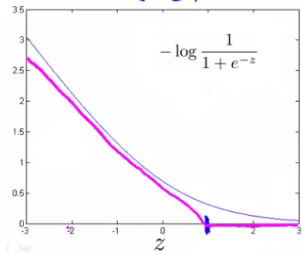
\includegraphics[width=\textwidth]{W7_1}
         \caption{}
         \label{fig:W7_1}
     \end{subfigure}
     \begin{subfigure}[b]{0.35\textwidth}
         \centering
         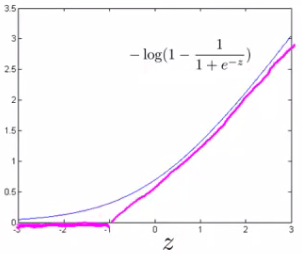
\includegraphics[width=\textwidth]{W7_2}
         \caption{}
         \label{fig:W7_2}
     \end{subfigure}
        \caption{}
        \label{fig:}
\end{figure}

We shall denote these as $\text{cost}_1(z)$ and $\text{cost}_0(z)$ (respectively, note that $\text{cost}_1(z)$ is the cost for classifying when y=1, and $\text{cost}_0(z)$ is the cost for classifying when y=0), and we may define them as follows (where k is an arbitrary constant defining the magnitude of the slope of the line):

$$z = \theta^Tx$$
$$\text{cost}_0(z) = \max(0, k(1+z))$$
$$\text{cost}_1(z) = \max(0, k(1-z))$$
Recall the full cost function from (regularized) logistic regression:
\begin{equation}
J(\theta) = \frac{1}{m} \sum_{i=1}^m y^{(i)}(-\log(h_\theta(x^{(i)}))) + (1 - y^{(i)})(-\log(1 - h_\theta(x^{(i)}))) + \dfrac{\lambda}{2m}\sum_{j=1}^n \Theta^2_jJ
\end{equation}
Note that the negative sign has been distributed into the sum in the above equation.

We may transform this into the cost function for support vector machines by substituting $\text{cost}_0(z)$ and $\text{cost}_1(z)$:

\begin{equation}
J(\theta) = \frac{1}{m} \sum_{i=1}^m y^{(i)} \ \text{cost}_1(\theta^Tx^{(i)}) + (1 - y^{(i)}) \ \text{cost}_0(\theta^Tx^{(i)}) + \dfrac{\lambda}{2m}\sum_{j=1}^n \Theta^2_j
\end{equation}

We can optimize this a bit by multiplying this by m (thus removing the m factor in the denominators). Note that this does not affect our optimization, since we're simply multiplying our cost function by a positive constant (for example, minimizing $(u-5)^2 + 1$ gives us 5; multiplying it by 10 to make it $10(u-5)^2 + 10$ still gives us 5 when minimized).
\begin{equation}
J(\theta) = \sum_{i=1}^m y^{(i)} \ \text{cost}_1(\theta^Tx^{(i)}) + (1 - y^{(i)}) \ \text{cost}_0(\theta^Tx^{(i)}) + \dfrac{\lambda}{2}\sum_{j=1}^n \Theta^2_j
\end{equation}

This is equivalent to multiplying the equation by $C = \dfrac{1}{\lambda}$, and thus results in the same values when optimized. Now, when we wish to regularize more (that is, reduce overfitting), we decrease C, and when we wish to regularize less (that is, reduce underfitting), we increase C.

Finally, note that the hypothesis of the Support Vector Machine is not interpreted as the probability of y being 1 or 0 (as it is for the hypothesis of logistic regression). Instead, it outputs either 1 or 0. (In technical terms, it is a discriminant function.)
\begin{equation}
h_\theta(x) = \begin{cases}1 & \text{if}\quad \Theta^Tx\ge0 \\0 &\text{if}\quad \text{otherwise}\end{cases}
\end{equation}

\section{Large Margin Intuition}
A useful way to think about Support Vector Machines is to think of them as Large Margin Classifiers.
\begin{itemize}
\item If y=1, we want $\Theta^Tx \geq 1$ (not just $\ge$ 0)
\item If y=0, we want $\Theta^Tx \leq 1$ (not just $<$ 0)
\end{itemize}

Now when we set our constant C to a very large value (e.g. 100,000), our optimizing function will constrain $\Theta$ such that the equation A (the summation of the cost of each example) equals 0. We impose the following constraints on $\Theta$:

$\Theta^Tx \geq 1$ if y=1 and $\Theta^Tx \leq -1$ if y=0.

If C is very large, we must choose $\Theta$ parameters such that:
\[\sum_{i=1}^m y^{(i)}\text{cost}_1(\Theta^Tx) + (1 - y^{(i)})\text{cost}_0(\Theta^Tx) = 0\]
This reduces our cost function to:
\begin{align*}
J(\theta) = C \cdot 0 + \dfrac{1}{2}\sum_{j=1}^n \Theta^2_j \newline
= \dfrac{1}{2}\sum_{j=1}^n \Theta^2_j
\end{align*}
Recall the decision boundary from logistic regression (the line separating the positive and negative examples). In SVMs, the decision boundary has the special property that it is \textbf{as far away as possible} from both the positive and the negative examples.

The distance of the decision boundary to the nearest example is called the \textbf{margin}. Since SVMs maximize this margin, it is often called a Large Margin Classifier.

The SVM will separate the negative and positive examples by a \textbf{large margin}.

This large margin is only achieved when C is very large.

Data is \textbf{linearly separable} when a \textbf{straight line} can separate the positive and negative examples.

If we have \textbf{outlier} examples that we don't want to affect the decision boundary, then we can \textbf{reduce} C.

Increasing and decreasing C is similar to respectively decreasing and increasing $\lambda$, and can simplify our decision boundary.
\section{Mathematics Behind Large Margin Classification}
\subsection{Vector Inner Product}
Say we have two vectors, u and v:

\begin{align*}
u = 
\begin{bmatrix}
u_1 \\ u_2
\end{bmatrix}
v = 
\begin{bmatrix}
v_1 \\ v_2
\end{bmatrix}
\end{align*}

The \textbf{length of vector v} is denoted $\parallel v\parallel$, and it describes the line on a graph from origin (0,0) to $(v_1,v_2)$

The length of vector v can be calculated with $\sqrt{v_1^2 + v_2^2}$ by the Pythagorean theorem.

The \textbf{projection} of vector v onto vector u is found by taking a right angle from u to the end of v, creating a right triangle.

\begin{itemize}
\item p = length of projection of v onto the vector u.
\item $u^Tv = p \cdot \parallel v \parallel$
\end{itemize}

Note that  $u^Tv = ||u|| \cdot ||v|| \cos \theta$ where $\theta$ is the angle between u and v. Also, $p = ||v|| \cos \theta$. If you substitute $p$ for $||v|| \cos \theta$ you get $u^Tv= p \cdot ||u||$.

So the product $u^Tv$ is equal to the length of the projection times the length of vector u.

In our example, since u and v are vectors of the same length, $u^Tv = v^Tu$.

$u^Tv = v^Tu = p \cdot ||u|| = u_1v_1 + u_2v_2$

If the \textbf{angle} between the lines for $v$ and $u$ is \textbf{greater than 90 degrees}, then the projection $p$ will be negative.
\begin{align*}
&\min_\Theta \dfrac{1}{2}\sum_{j=1}^n \Theta_j^2 \\
&= \dfrac{1}{2}(\Theta_1^2 + \Theta_2^2 + \dots + \Theta_n^2) \\
&= \dfrac{1}{2}(\sqrt{\Theta_1^2 + \Theta_2^2 + \dots + \Theta_n^2})^2 \\
&= \dfrac{1}{2}||\Theta ||^2 \\
\end{align*}

We can use the same rules to rewrite $\Theta^Tx^{(i)}$
\[
\Theta^Tx^{(i)} = p^{(i)} \cdot ||\Theta || = \Theta_1x_1^{(i)} + \Theta_2x_2^{(i)} + \dots + \Theta_n x_n^{(i)}
\]

So we now have a new optimization objective by substituting $p^{(i)} \cdot ||\Theta ||$ in for $\Theta^Tx^{(i)}$
\begin{itemize}
\item If y=1, we want $p^{(i)} \cdot ||\Theta || \geq 1$
\item If y=0, we want $p^{(i)} \cdot ||\Theta || \leq -1$
\end{itemize}

The reason this causes a ``large margin" is because: the vector for $\Theta$ is perpendicular to the decision boundary. In order for our optimization objective (above) to hold true, we need the absolute value of our projections $p^{(i)}$ to be as large as possible.

If $\Theta_0 =0$, then all our decision boundaries will intersect (0,0). If $\Theta_0 \neq 0$, the support vector machine will still find a large margin for the decision boundary.

\section{Kernels I}
Kernels allow us to make complex, non-linear classifiers using Support Vector Machines.

Given x, compute new feature depending on proximity to landmarks $l^{(1)},\ l^{(2)},\ l^{(3)}$

To do this, we find the ``similarity" of $x$ and some landmark $l^{(i)}$s:
\[
f_i = similarity(x, l^{(i)}) = \exp(-\dfrac{\sum^n_{j=1}(x_j-l_j^{(i)})^2}{2\sigma^2})
\]

There are a couple properties of the similarity function:

If $x \approx l^{(i)}$), then $f_i = \exp(-\dfrac{\approx 0^2}{2\sigma^2}) \approx 1$

If x is far from $l^{(i)}$, then $f_i = \exp(-\dfrac{(large\ number)^2}{2\sigma^2}) \approx 0$

In other words, if x and the landmark are close, then the similarity will be close to 1, and if x and the landmark are far away from each other, the similarity will be close to 0.

Each landmark gives us the features in our hypothesis:


\begin{align*}l^{(1)} \rightarrow f_1 \newline l^{(2)} \rightarrow f_2 \\
 l^{(3)} \rightarrow f_3 \\
\dots \\
 h_\Theta(x) = \Theta_1f_1 + \Theta_2f_2 + \Theta_3f_3 + \dots
\end{align*}

$\sigma^2$is a parameter of the Gaussian Kernel, and it can be modified to increase or decrease the \textbf{drop-off} of our feature $f_i$. Combined with looking at the values inside $\Theta$, we can choose these landmarks to get the general shape of the decision boundary.

\section{Kernels II}
One way to get the landmarks is to put them in the \textbf{exact same} locations as all the training examples. This gives us m landmarks, with one landmark per training example.

Given example x:

$f_1 = similarity(x,l^{(1)})$, $f_2 = similarity(x,l^{(2)})$, $f_3 = similarity(x,l^{(3)})$, and so on.

This gives us a ``feature vector", $f_{(i)}$ of all our features for example $x_{(i)}$. We may also set $f_0 = 1$ to correspond with $\Theta_0$. Thus given training example $x_{(i)}$:

$$x^{(i)} \rightarrow f^{(i)}_1=similarity(x^{(i)},l^{(1)})f^{(i)}_2$$
$$=similarity(x^{(i)},l^{(2)})\cdots f^{(i)}_m$$
$$=similarity(x^{(i)},l^{(m)})$$

Now to get the parameters Θ we can use the \textbf{SVM} minimization algorithm but with $f^{(i)}$ substituted in for $x^{(i)}$:
$$
\min_{\Theta} C \sum_{i=1}^m y^{(i)}\text{cost}_1(\Theta^Tf^{(i)}) + (1 - y^{(i)})\text{cost}_0(\theta^Tf^{(i)}) + \dfrac{1}{2}\sum_{j=1}^n \Theta^2_j
$$
Using kernels to generate f(i) is not exclusive to SVMs and may also be applied to logistic regression. However, because of computational optimizations on SVMs, kernels combined with SVMs is much faster than with other algorithms, so kernels are almost always found combined only with SVMs.
\subsection{Choosing SVM parameters}
Choosing C (recall that $C = \dfrac{1}{\lambda}$)
\begin{itemize}
\item If C is large, then we get higher variance/lower bias
\item If C is small, then we get lower variance/higher bias
\end{itemize}

The other parameter we must choose is $\sigma^2$ from the Gaussian Kernel function:
\begin{itemize}
\item With a large $\sigma^2$, the features fi vary more smoothly, causing higher bias and lower variance.
\item With a small $\sigma^2$, the features fi vary less smoothly, causing lower bias and higher variance.
\end{itemize}

\subsection{Using An SVM}

There are lots of good SVM libraries already written. A. Ng often uses `\textbf{liblinear}' and `\textbf{libsvm}'. In practical application, you should use one of these libraries rather than rewrite the functions.

In practical application, the choices you do need to make are:
\begin{itemize}
\item Choice of parameter C
\teim Choice of kernel (similarity function)
\item No kernel (``linear" kernel) -- gives standard linear classifier
\item Choose when n is large and when m is small
\item Gaussian Kernel (above) -- need to choose $\sigma^2$ 
\item Choose when n is small and m is large
\end{itemize}

The library may ask you to provide the kernel function.

\textbf{Note}: do perform feature scaling before using the Gaussian Kernel.

\textbf{Note}: not all similarity functions are valid kernels. They must satisfy ``Mercer's Theorem" which guarantees that the SVM package's optimizations run correctly and do not diverge.

You want to train C and the parameters for the kernel function using the training and cross-validation datasets.

\subsection{Multi-class Classification}
Many SVM libraries have multi-class classification built-in.

You can use the one-vs-all method just like we did for logistic regression, where $y \in {1,2,3,\dots,K}$ with $\Theta^{(1)}, \Theta^{(2)}, \dots,\Theta{(K)}$. We pick class $i$ with the largest ($\Theta^{(i)})^Tx$.

\subsection{Logistic Regression vs. SVMs}
If n is large (relative to m), then use logistic regression, or SVM without a kernel (the ``linear kernel")

If n is small and m is intermediate, then use SVM with a Gaussian Kernel

If n is small and m is large, then manually create/add more features, then use logistic regression or SVM without a kernel.

In the first case, we don't have enough examples to need a complicated polynomial hypothesis. In the second example, we have enough examples that we may need a complex non-linear hypothesis. In the last case, we want to increase our features so that logistic regression becomes applicable.

\textbf{Note}: a neural network is likely to work well for any of these situations, but may be slower to train.

\subsubsection{Additional references}
\begin{itemize}
\item \href{http://web.mit.edu/6.034/wwwbob/svm-notes-long-08.pdf}{An Idiot's Guide to Support Vector Machines}
\end{itemize}